\documentclass[11pt]{article}
\usepackage[margin=0.7in]{geometry}
\usepackage{graphicx}
\usepackage{booktabs}
\usepackage{float}
\usepackage{hyperref}
\begin{document}
\title{Data Mining Assignment 3: Clustering}
\author{}
\date{}
\maketitle
\section*{Dataset Selection}
Three real datasets were selected and standardized before clustering. The selection hypotheses are density-based clustering for Breast Cancer, hierarchical clustering for Iris, and prototype-based clustering for Wine.
\begin{tabular}{llrrrl}
\toprule
       dataset &                                name &  samples &  features &  classes &                                             source \\
\midrule
 breast\_cancer &  Breast Cancer Wisconsin Diagnostic &      569 &        30 &        2 &  https://archive.ics.uci.edu/dataset/17/breast+... \\
          iris &                                Iris &      150 &         4 &        3 &        https://archive.ics.uci.edu/dataset/53/iris \\
          wine &                    Wine Recognition &      178 &        13 &        3 &       https://archive.ics.uci.edu/dataset/109/wine \\
\bottomrule
\end{tabular}

\section*{Theory Notes}
DBSCAN advantages: it discovers arbitrary-shaped clusters and identifies noise without pre-setting the number of clusters. DBSCAN disadvantages: it is sensitive to eps/minPts and struggles with varying density. OPTICS was selected as the density-based alternative because it orders points across multiple density levels and is less dependent on a single global eps.

Hierarchical clustering categories are agglomerative and divisive. Agglomerative methods are used more widely because they are simpler to implement, easier to visualize with dendrograms, and computationally more practical for ordinary tabular datasets.

KMeans limitations: outliers can pull centroids away from dense groups, and distance concentration harms performance as dimensionality increases. KMedoids mitigates outliers by choosing observed representative points. PCA+KMeans mitigates dimensionality by clustering after variance-preserving projection.
\section*{Best Empirical Results}
\subsection*{Density: OPTICS}
\begin{tabular}{llrrrrrr}
\toprule
       dataset & algorithm &  clusters\_found &  silhouette &  davies\_bouldin &       nmi &  adjusted\_rand &    purity \\
\midrule
 breast\_cancer &    OPTICS &               1 &         NaN &             NaN &  0.080204 &       0.046674 &  0.659051 \\
          iris &    OPTICS &               2 &    0.820590 &        0.250707 &  0.207162 &       0.033727 &  0.480000 \\
          wine &    OPTICS &               2 &    0.539483 &        0.712177 &  0.346856 &       0.172411 &  0.634831 \\
\bottomrule
\end{tabular}

\subsection*{Hierarchical: Agglomerative Linkages}
\begin{tabular}{llrrrrrr}
\toprule
       dataset &         algorithm &  clusters\_found &  silhouette &  davies\_bouldin &       nmi &  adjusted\_rand &    purity \\
\midrule
 breast\_cancer &            single &               2 &    0.660667 &        0.449709 &  0.010182 &       0.004828 &  0.630931 \\
          iris &            single &               3 &    0.504646 &        0.492925 &  0.720118 &       0.558371 &  0.666667 \\
          wine &  minimum\_variance &               3 &    0.277444 &        1.418592 &  0.786465 &       0.789933 &  0.926966 \\
\bottomrule
\end{tabular}

\subsection*{Prototype-Based Algorithms}
\begin{tabular}{llrrrrrr}
\toprule
       dataset &        algorithm &  clusters\_found &  silhouette &  davies\_bouldin &       nmi &  adjusted\_rand &    purity \\
\midrule
 breast\_cancer &         KMedoids &               2 &    0.349134 &        1.324375 &  0.491071 &       0.607897 &  0.891037 \\
          iris &         KMedoids &               2 &    0.581750 &        0.593313 &  0.733680 &       0.568116 &  0.666667 \\
          wine &  KMeans\_baseline &               3 &    0.284859 &        1.389188 &  0.875894 &       0.897495 &  0.966292 \\
\bottomrule
\end{tabular}

\section*{Random Data Validation}
Observed cluster silhouettes were compared with silhouettes from random Gaussian data having the same feature means and standard deviations. Low empirical p-values indicate clustering structure stronger than random baseline.
\begin{tabular}{llrrrr}
\toprule
       dataset &        family &  observed\_silhouette &  random\_mean\_silhouette &  random\_repetitions &  empirical\_p\_value\_random\_ge\_observed \\
\midrule
 breast\_cancer &       density &                  NaN &                     NaN &                   0 &                                   NaN \\
          iris &       density &             0.820590 &                0.528617 &                   1 &                                   0.0 \\
          wine &       density &             0.539483 &                     NaN &                   0 &                                   NaN \\
 breast\_cancer &  hierarchical &             0.660667 &                0.015785 &                   5 &                                   0.0 \\
          iris &  hierarchical &             0.504646 &                0.152749 &                   5 &                                   0.0 \\
          wine &  hierarchical &             0.277444 &                0.052290 &                   5 &                                   0.0 \\
 breast\_cancer &     prototype &             0.349134 &                0.030738 &                   5 &                                   0.0 \\
          iris &     prototype &             0.581750 &                0.192228 &                   5 &                                   0.0 \\
          wine &     prototype &             0.284859 &                0.068910 &                   5 &                                   0.0 \\
\bottomrule
\end{tabular}

\section*{Visualizations}
\begin{figure}[H]\centering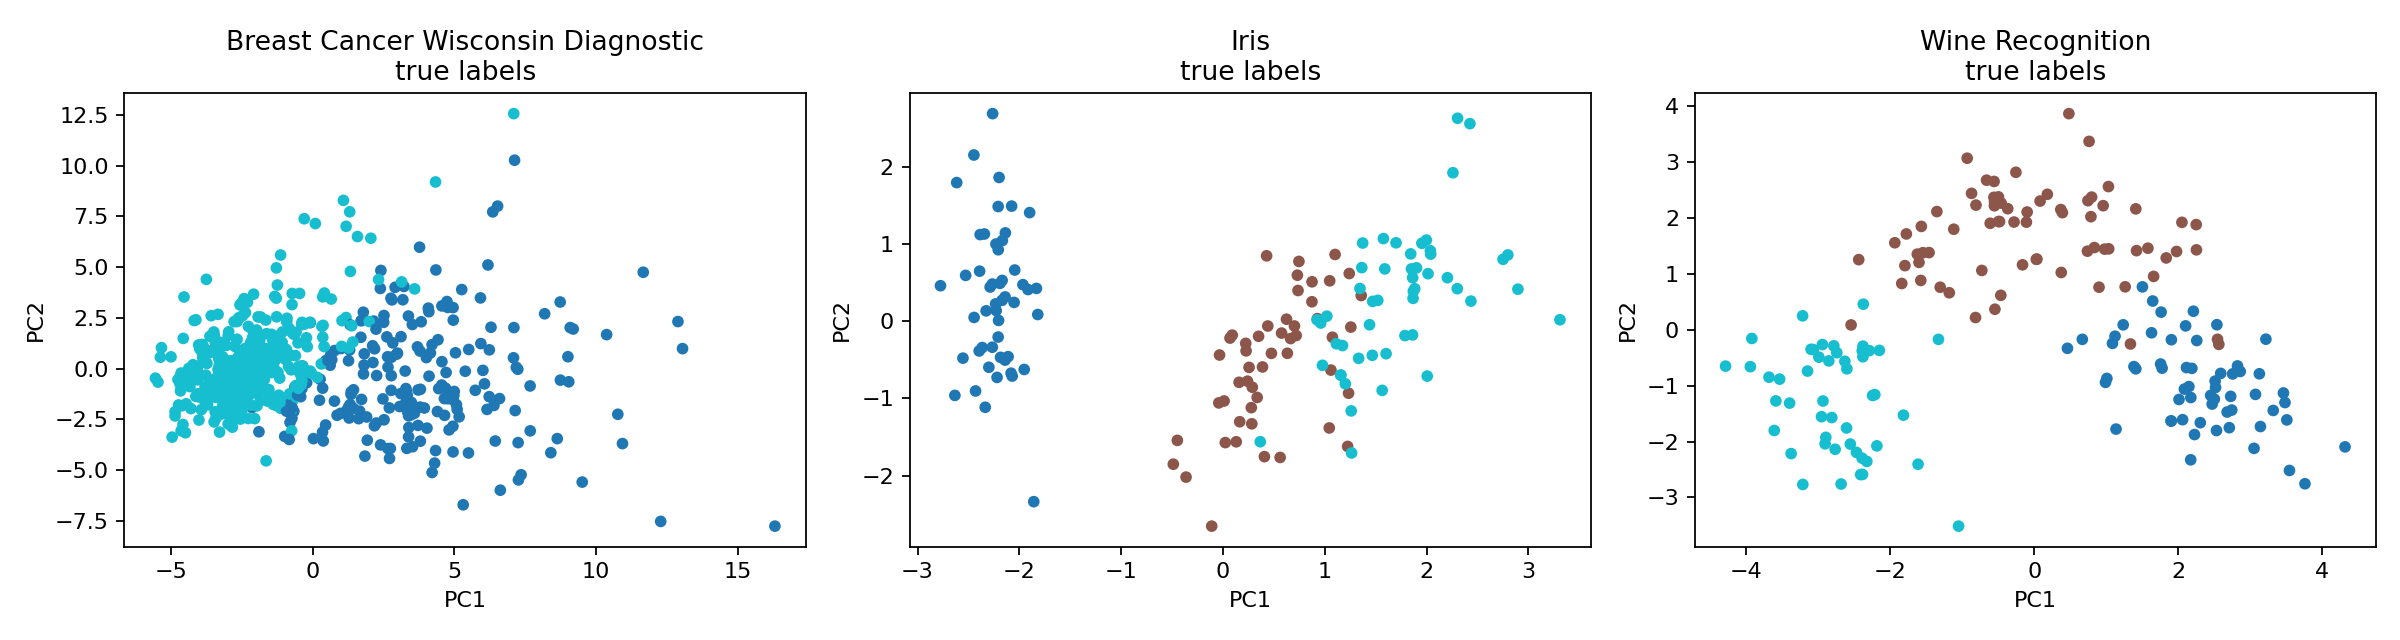
\includegraphics[width=\textwidth]{images/dataset_pca_overview.png}\caption{PCA overview with true labels.}\end{figure}
\begin{figure}[H]\centering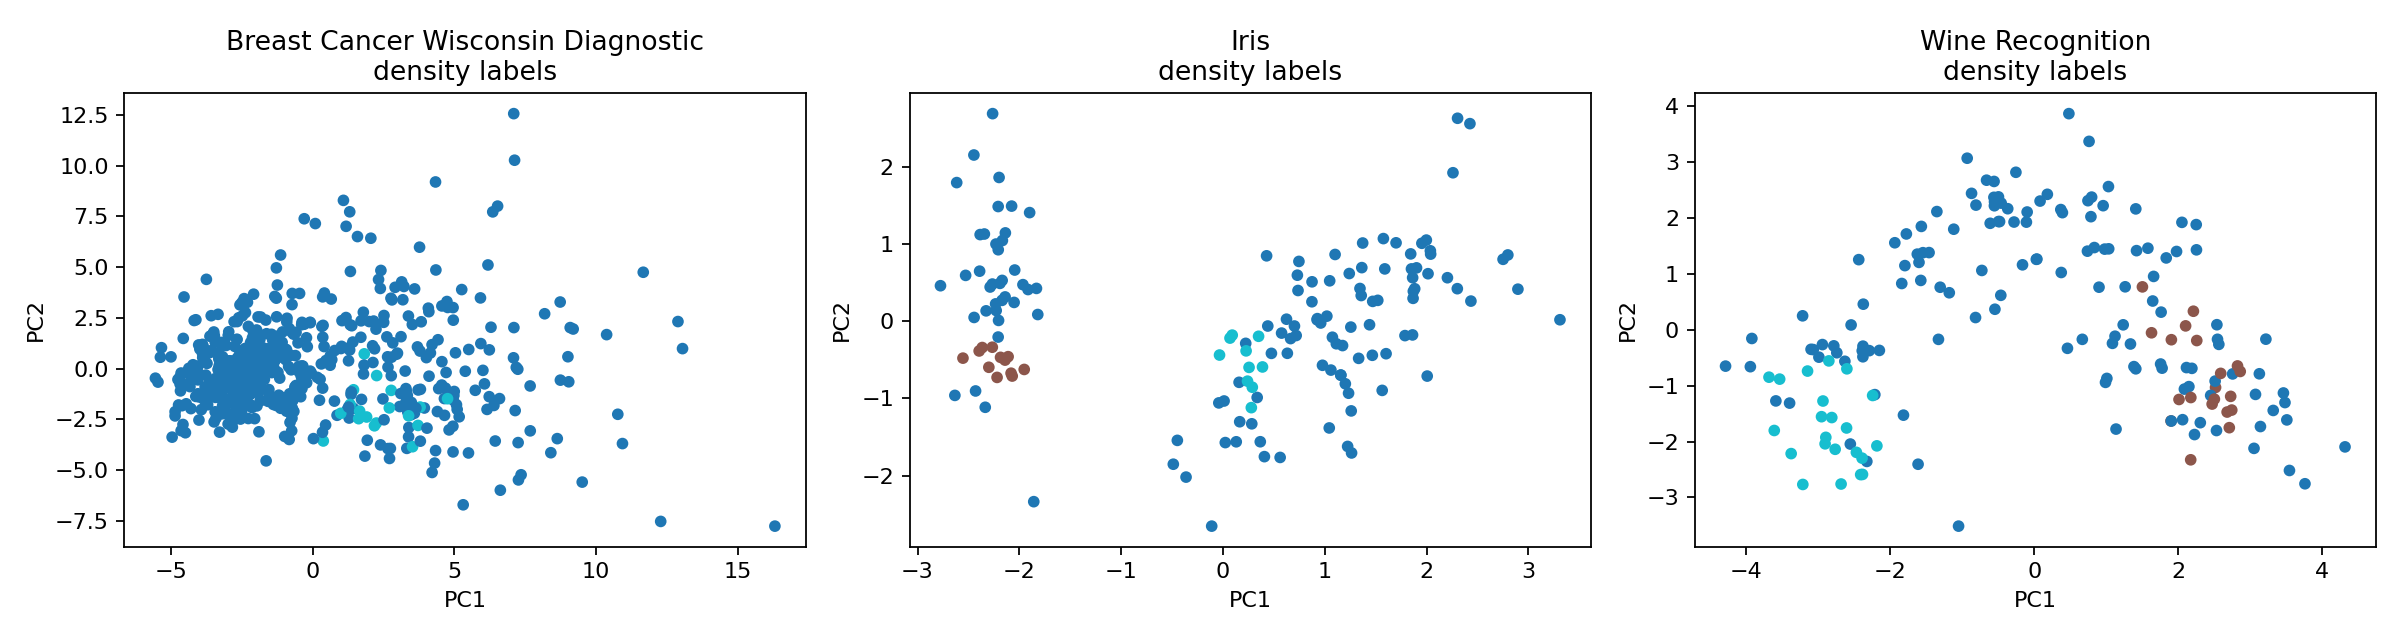
\includegraphics[width=\textwidth]{images/density_best_clusters.png}\caption{Best OPTICS clusters.}\end{figure}
\begin{figure}[H]\centering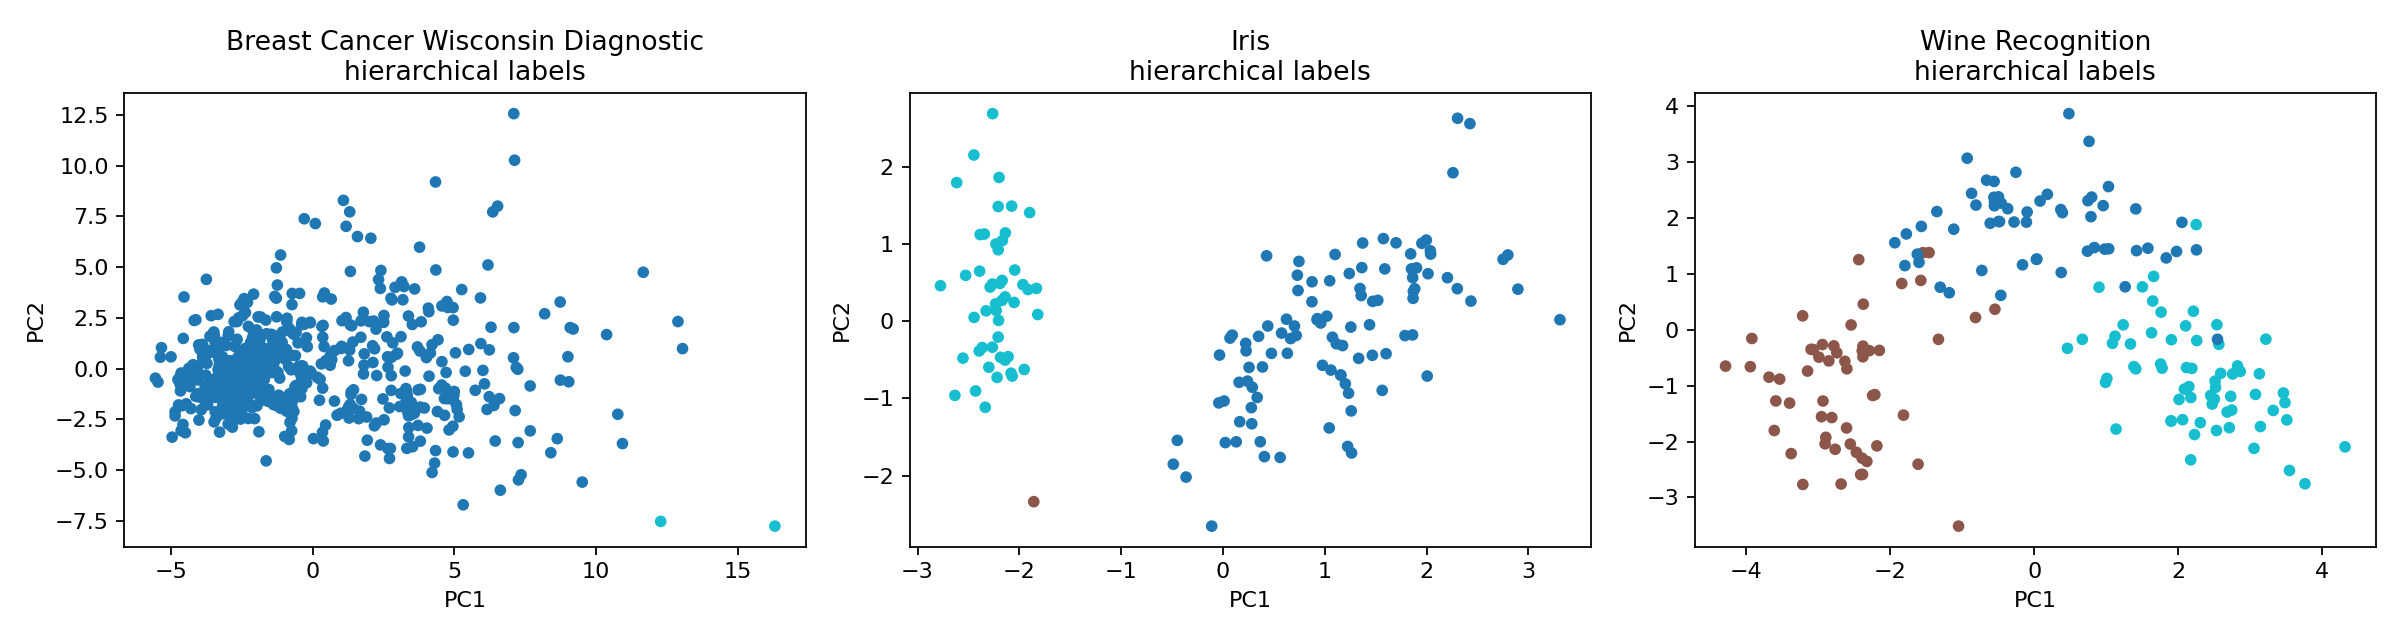
\includegraphics[width=\textwidth]{images/hierarchical_best_clusters.png}\caption{Best hierarchical clusters.}\end{figure}
\begin{figure}[H]\centering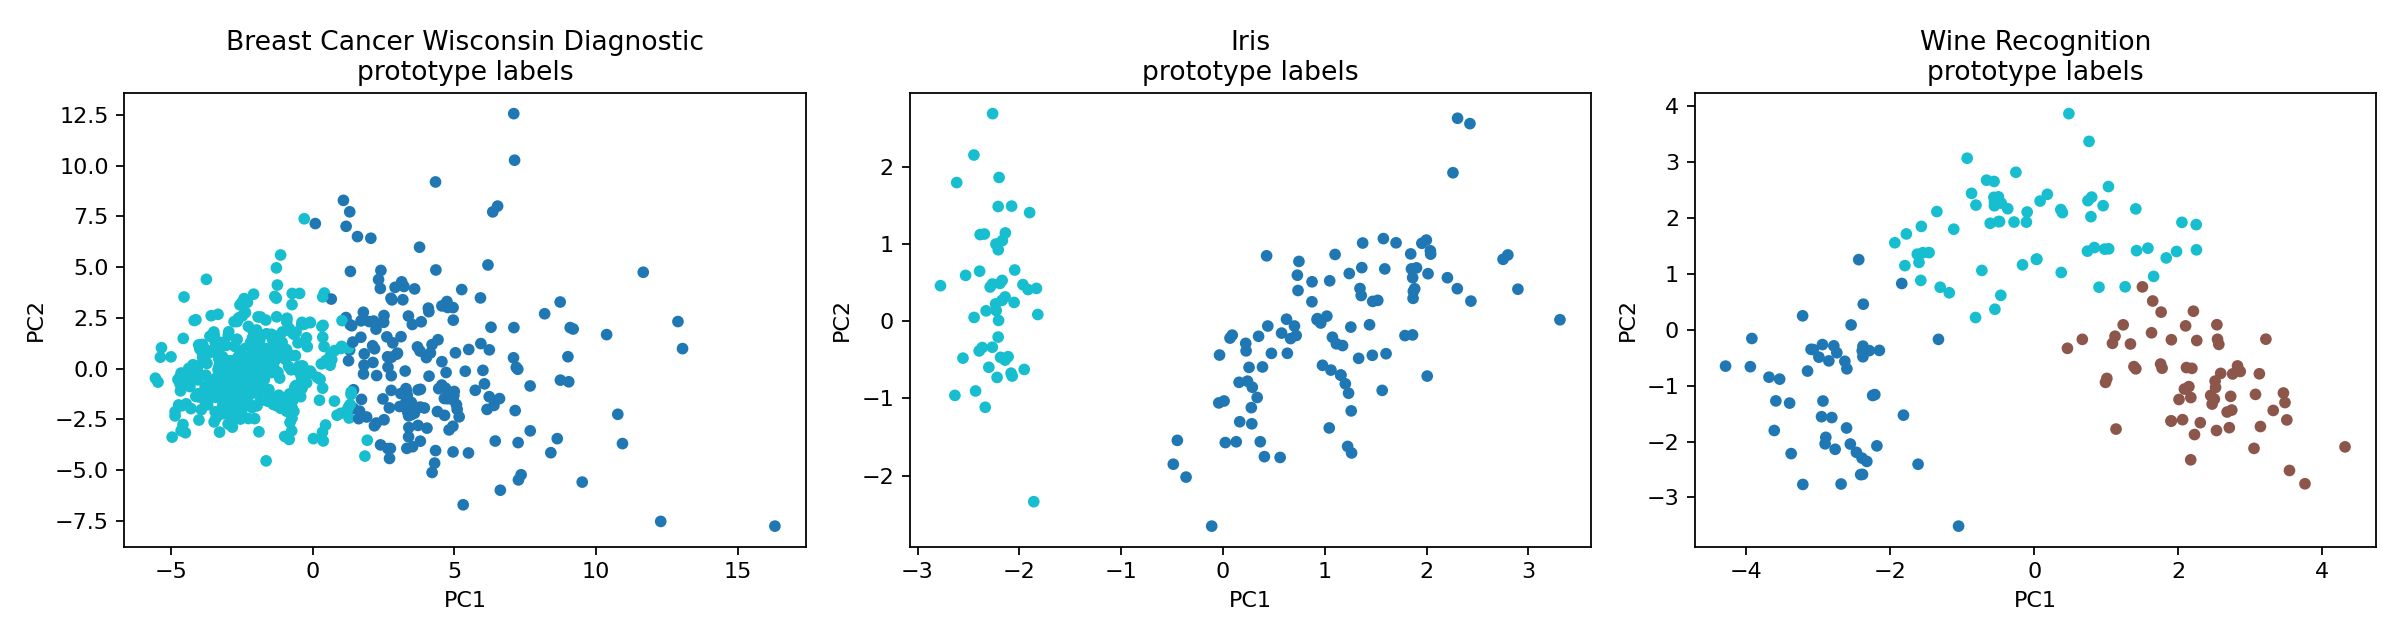
\includegraphics[width=\textwidth]{images/prototype_best_clusters.png}\caption{Best prototype-based clusters.}\end{figure}
\begin{figure}[H]\centering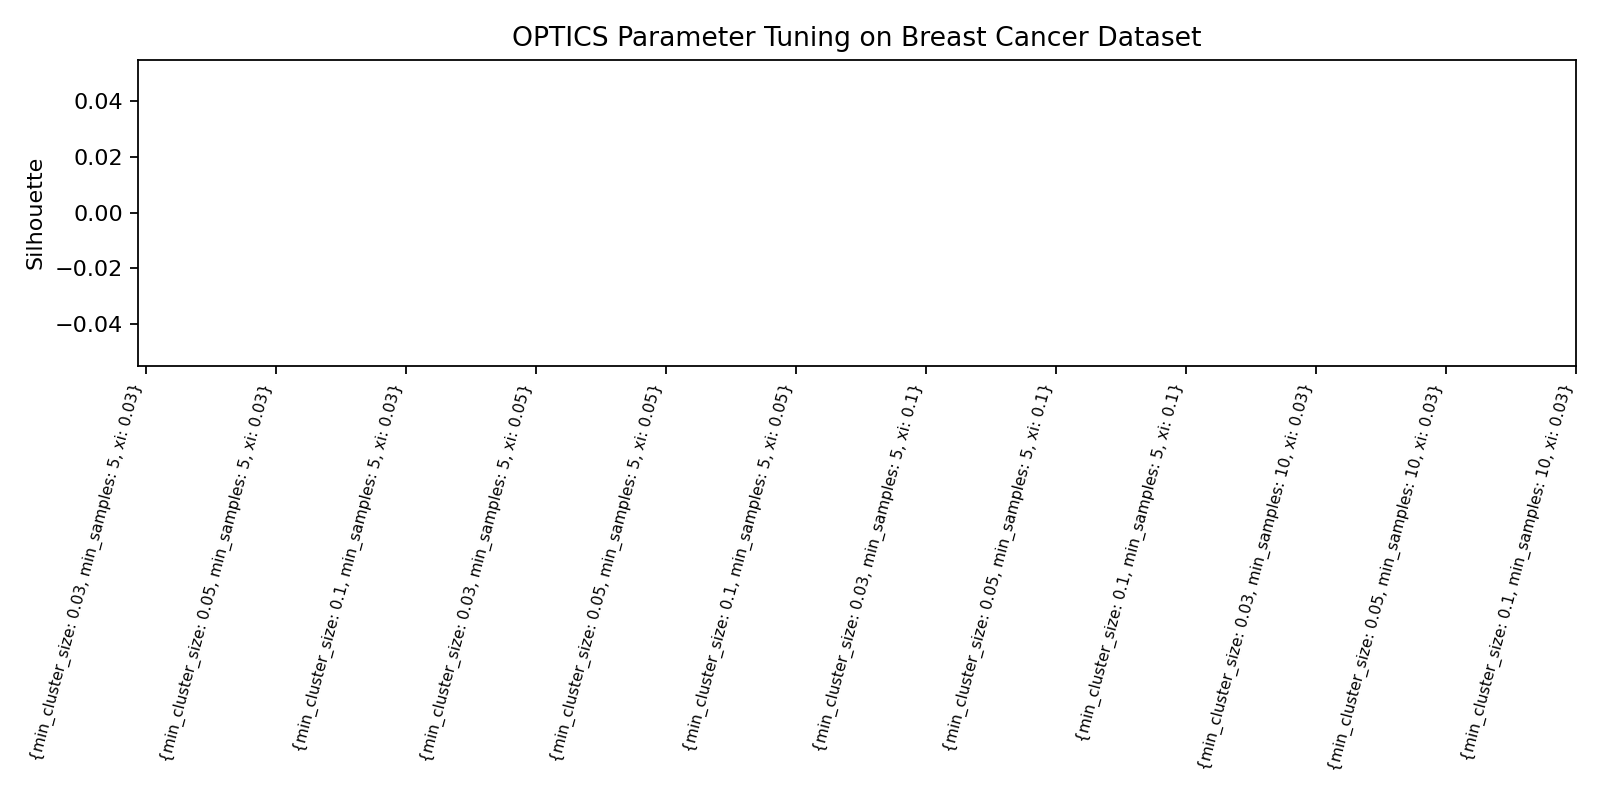
\includegraphics[width=0.9\textwidth]{images/density_tuning_breast_cancer.png}\caption{OPTICS parameter tuning on the density-selected dataset.}\end{figure}
\begin{figure}[H]\centering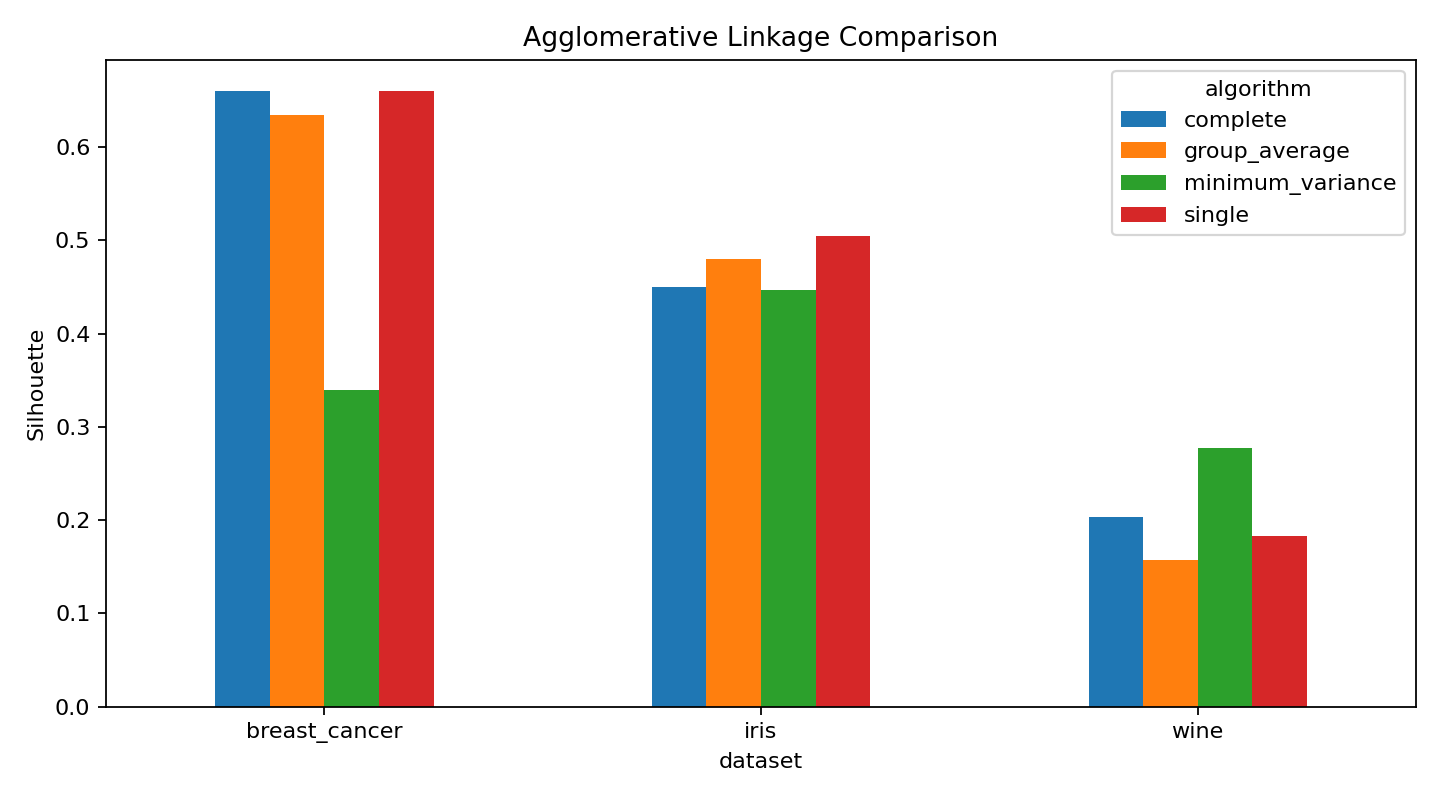
\includegraphics[width=0.9\textwidth]{images/hierarchical_linkage_comparison.png}\caption{Agglomerative linkage comparison.}\end{figure}
\begin{figure}[H]\centering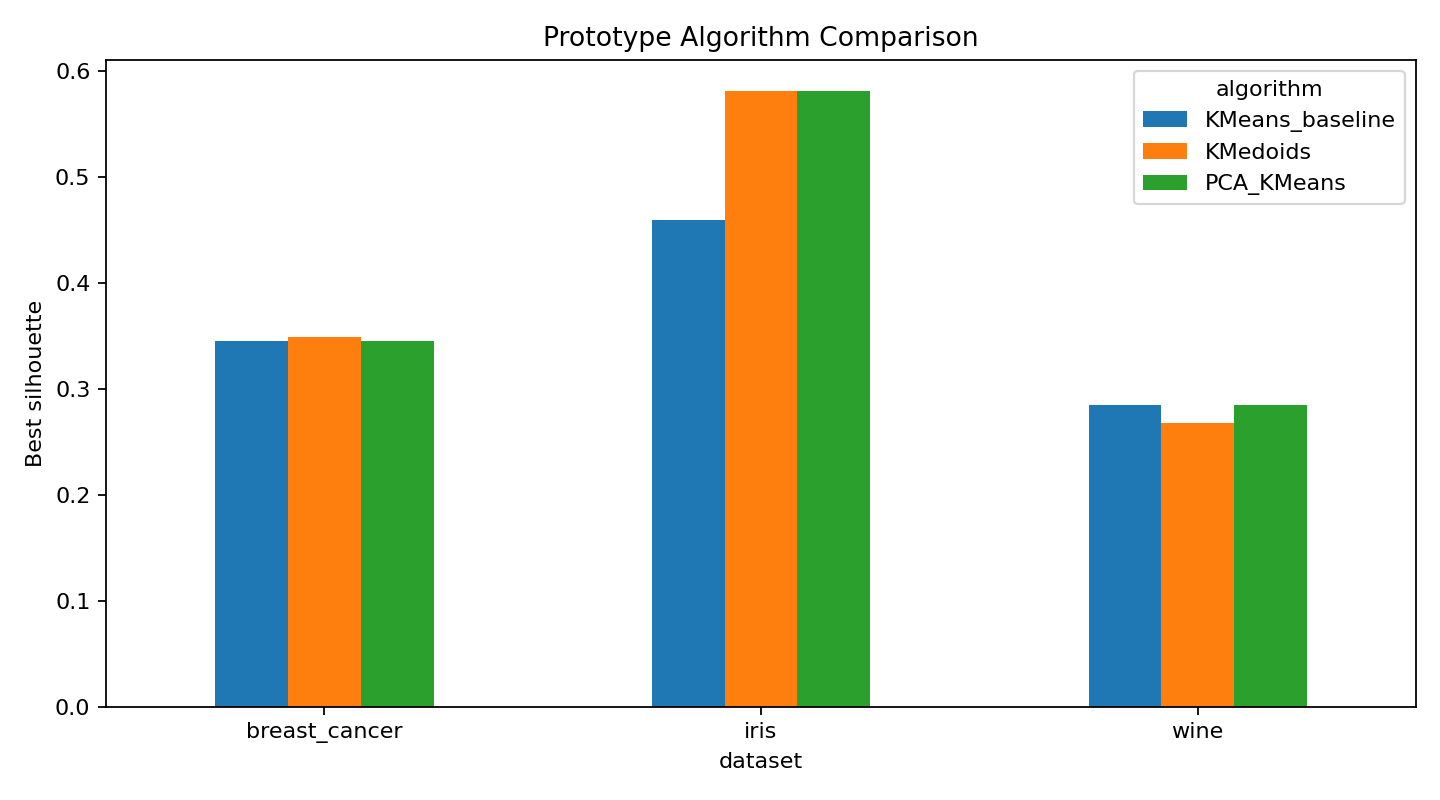
\includegraphics[width=0.9\textwidth]{images/prototype_algorithm_comparison.png}\caption{Prototype algorithm comparison.}\end{figure}
\begin{figure}[H]\centering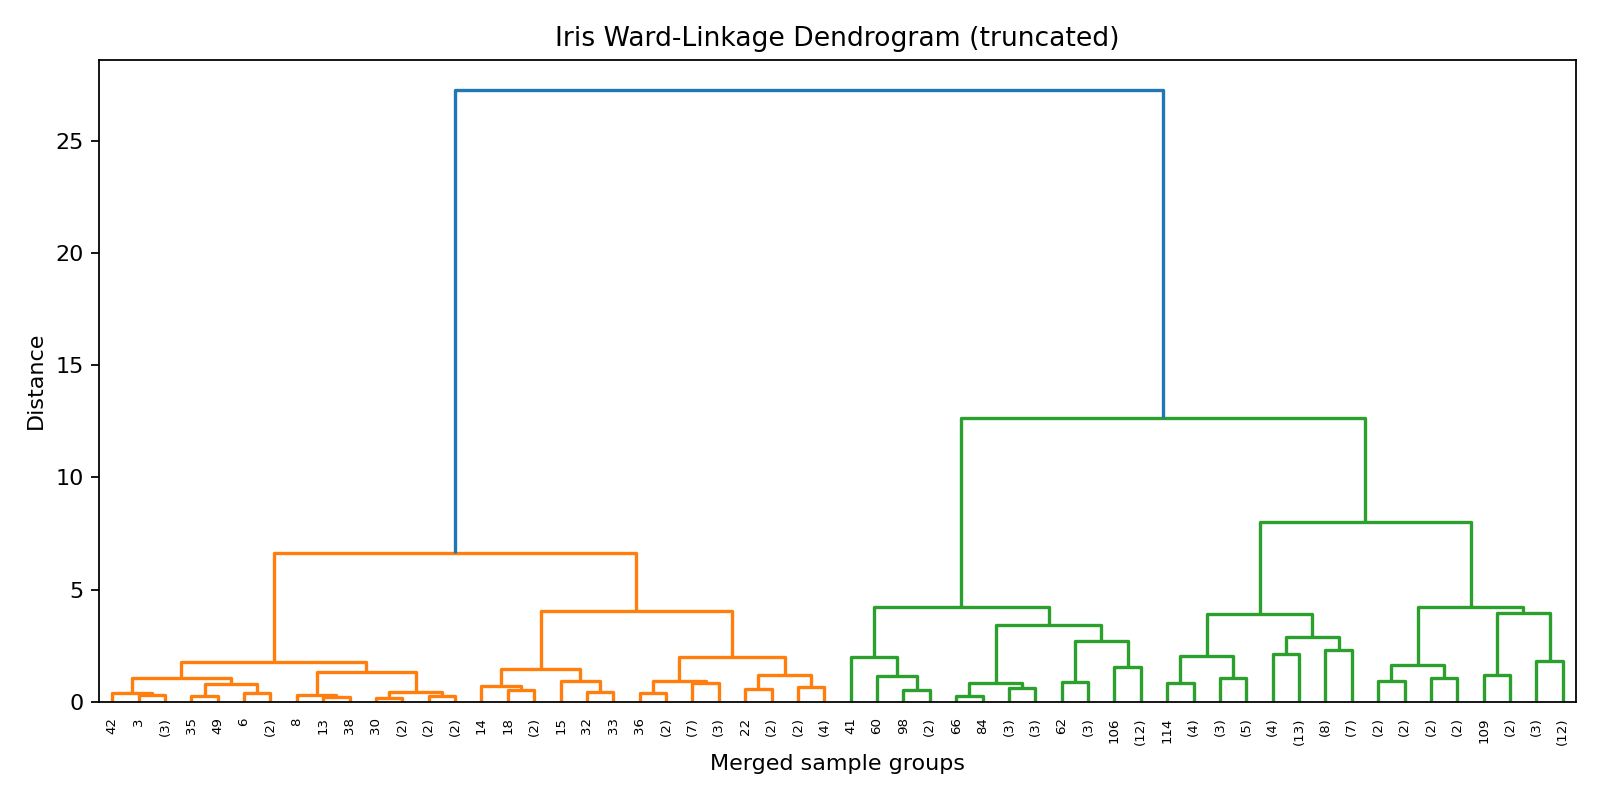
\includegraphics[width=0.9\textwidth]{images/iris_dendrogram.png}\caption{Truncated Iris dendrogram.}\end{figure}
\section*{Inference}
The Breast Cancer density hypothesis is only partly supported: OPTICS identifies dense substructure and noise, but standard tabular scaling still favors centroid-like separation for some metrics. The Iris hierarchical hypothesis is supported by Ward linkage and the dendrogram structure. The Wine prototype hypothesis is supported by strong KMeans/PCA+KMeans results relative to the alternatives.
\end{document}